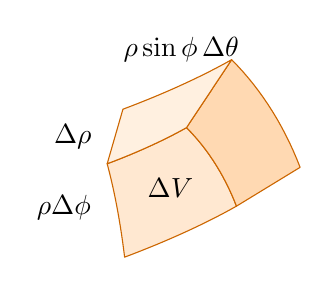
\begin{tikzpicture}[
    scale=1.1,
    line cap=round,
    line join=round,
    declare function={
        sx(\r,\t,\p) = \r*sin(\p)*(-0.6*cos(\t) + sin(\t));
        sy(\r,\t,\p) = \r*(cos(\p) + sin(\p)*(-0.45*cos(\t) + 0.15*sin(\t)));
    }
]
    % Draw three curved faces of a small spherical wedge.
    \filldraw[fill=orange!18,draw=orange!80!black]
        plot[domain=45:75,samples=16] ({sx(2.7,\x,40)},{sy(2.7,\x,40)})
        -- plot[domain=40:65,samples=16] ({sx(2.7,75,\x)},{sy(2.7,75,\x)})
        -- plot[domain=75:45,samples=16] ({sx(2.7,\x,65)},{sy(2.7,\x,65)})
        -- plot[domain=65:40,samples=16] ({sx(2.7,45,\x)},{sy(2.7,45,\x)}) -- cycle;
    \filldraw[fill=orange!30,draw=orange!80!black]
        ({sx(2.7,75,40)},{sy(2.7,75,40)})
        -- ({sx(3.7,75,40)},{sy(3.7,75,40)})
        -- plot[domain=40:65,samples=16] ({sx(3.7,75,\x)},{sy(3.7,75,\x)})
        -- ({sx(2.7,75,65)},{sy(2.7,75,65)})
        -- plot[domain=65:40,samples=16] ({sx(2.7,75,\x)},{sy(2.7,75,\x)}) -- cycle;
    \filldraw[fill=orange!12,draw=orange!80!black]
        ({sx(2.7,45,40)},{sy(2.7,45,40)})
        -- ({sx(3.7,45,40)},{sy(3.7,45,40)})
        -- plot[domain=45:75,samples=16] ({sx(3.7,\x,40)},{sy(3.7,\x,40)})
        -- ({sx(2.7,75,40)},{sy(2.7,75,40)})
        -- plot[domain=75:45,samples=16] ({sx(2.7,\x,40)},{sy(2.7,\x,40)}) -- cycle;
    % Label only the three local side lengths and the volume element.
    \path ({sx(2.7,45,40)},{sy(2.7,45,40)})
        -- ({sx(3.7,45,40)},{sy(3.7,45,40)}) node[midway,left=5pt] {$\Delta\rho$};
    \node[left=6pt] at ({sx(2.7,45,52.5)},{sy(2.7,45,52.5)}) {$\rho\Delta\phi$};
    \node[above=5pt] at ({sx(3.7,60,40)},{sy(3.7,60,40)}) {$\rho\sin\phi\,\Delta\theta$};
    \node at ({sx(2.7,60,53)},{sy(2.7,60,53)}) {$\Delta V$};
\end{tikzpicture}
